\section{Experimental Results}
\label{sec:result}

This section presents the experimental results and the answers to the RQs. 
More results are available at the \tool repository.\footnote{\href{https://github.com/csresearcher27/s2lct_project}{https://github.com/csresearcher27/s2lct$\_$project}} 
% \sw{@Jaeseong: footnote typically goes after punctuation, without space. I fix these; just wanted to let you know.}

\InputWithSpace{tables/test-results-all-table}
% \InputWithSpace{tables/test-results-table}
% \InputWithSpace{tables/test-results-3-50-table}
% \InputWithSpace{tables/test-results-3-100-table}
% \InputWithSpace{tables/test-results-3-200-table}
\InputWithSpace{tables/test-results-hs-table}

\begin{figure}
    \centering
    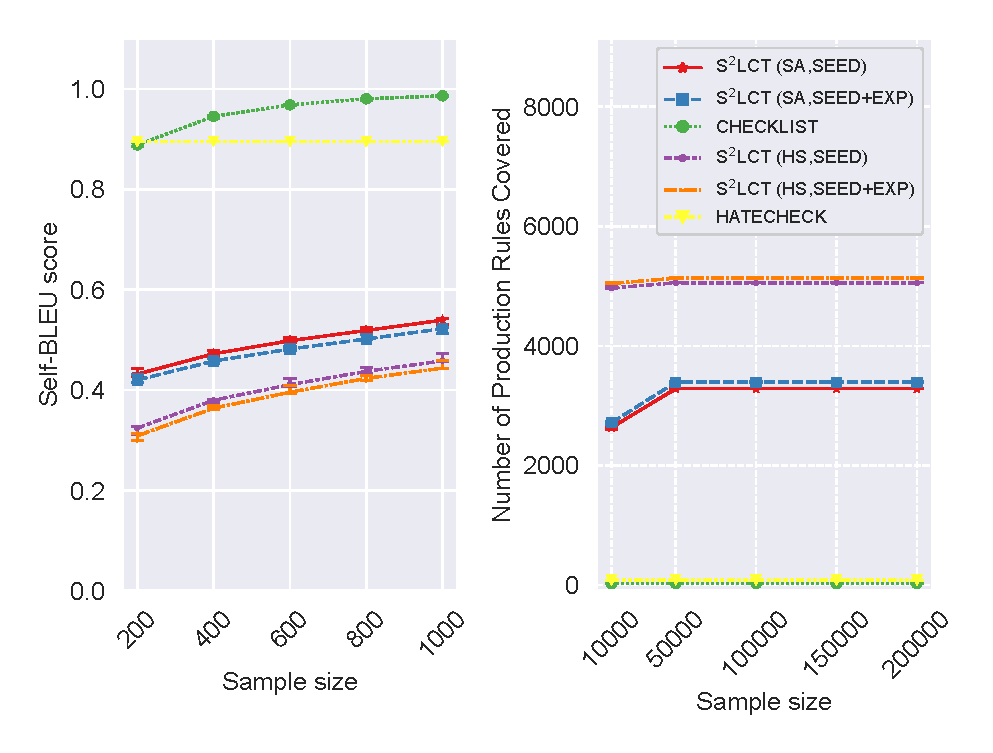
\includegraphics[width=0.35\textwidth]{figs/pdr-selfbleu-agg-lc-task-agg-lineplot.eps}
    \vspace{-3mm}
    \caption{\PdrSelfbleuFigCaption}
\end{figure}

\begin{figure}
    \centering
    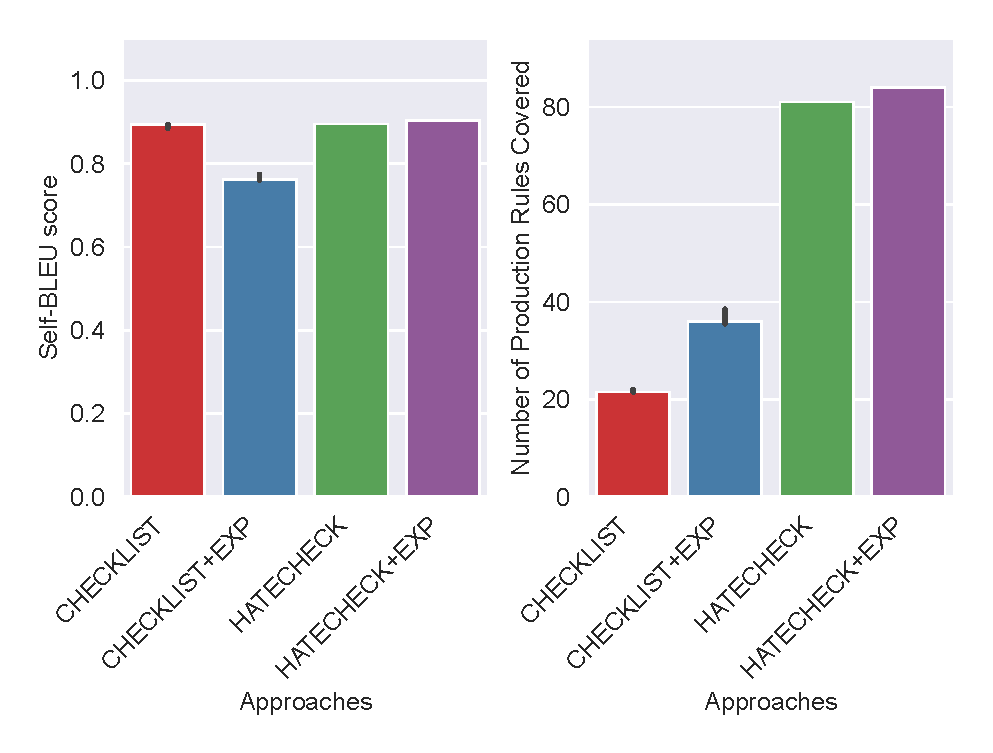
\includegraphics[width=0.3\textwidth]{figs/pdr-selfbleu-ablation-lc-task-agg-barplot.eps}
    \vspace{-3mm}
    \caption{\PdrSelfbleuBarplotFigCaption}
\end{figure}

\InputWithSpace{tables/mtnlp-comp-table}
\InputWithSpace{tables/adv-comp-table}

% \begin{figure}%
%     \centering
%     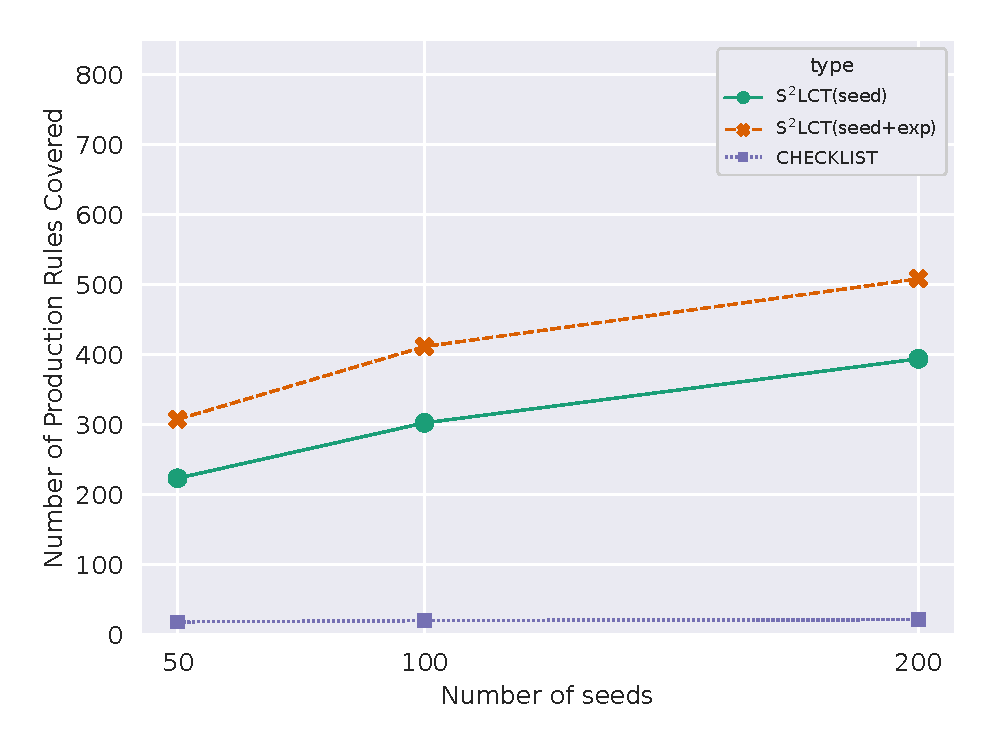
\includegraphics[width=0.35\textwidth]{figs/pdr-agg-lineplot.eps}
%     \caption{\PdrFigCaption}
% \end{figure}


% \begin{figure}%
%     \centering
%     \subfloat[][\centering\SelfbleuFigCaption]{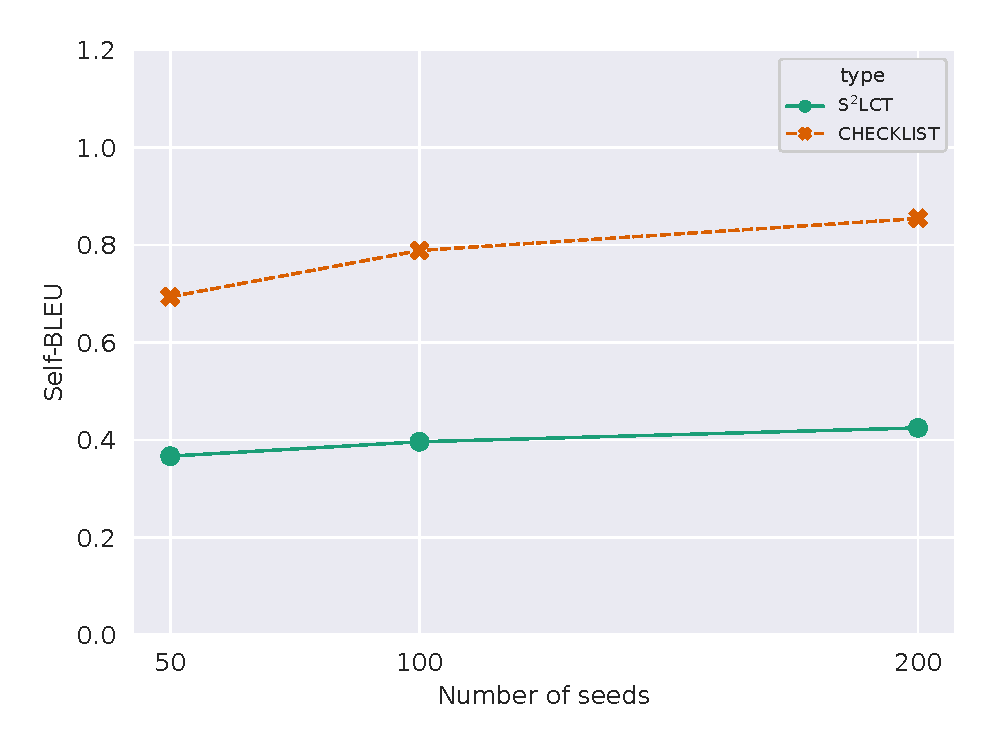
\includegraphics[width=0.35\textwidth]{figs/selfbleu-agg-sample-lineplot.eps}}%
%     \qquad
%     \subfloat[][\centering\PdrFigCaption]{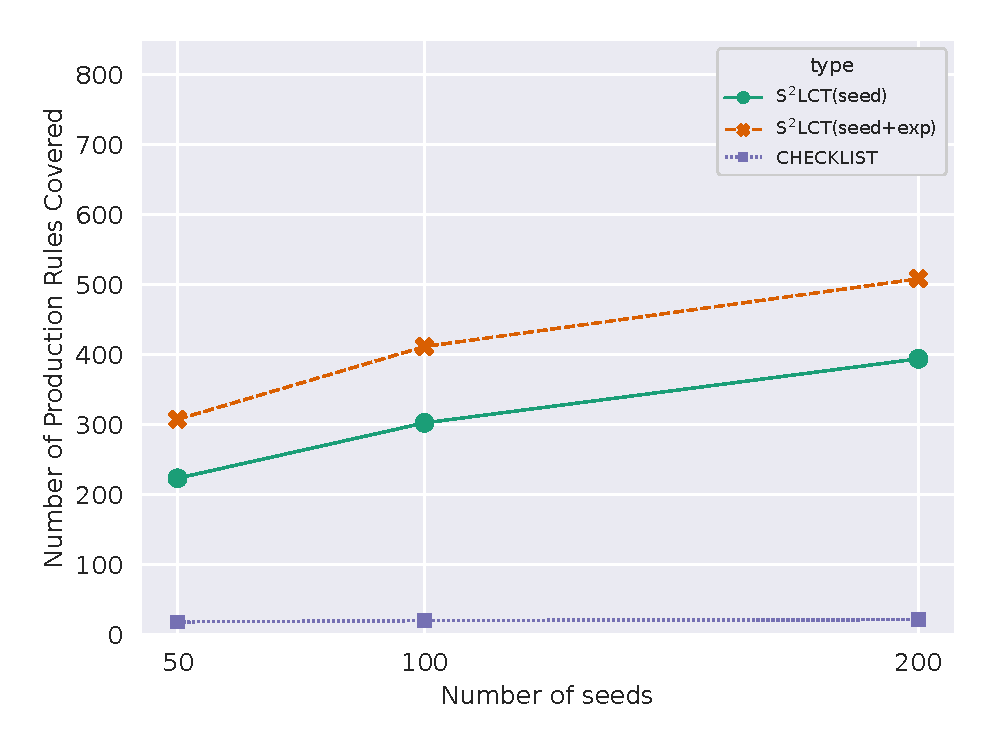
\includegraphics[width=0.35\textwidth]{figs/pdr-agg-lineplot.eps}}
%     \caption{\FailModelsFigCaption}
% \end{figure}

% \begin{figure}%
%     \centering
%     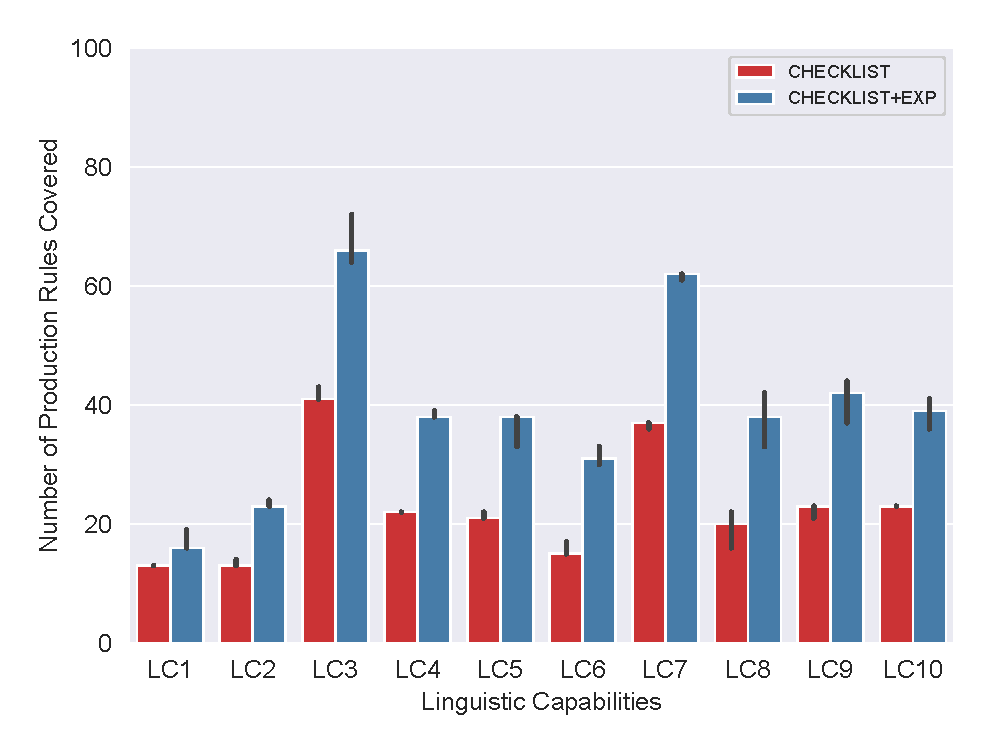
\includegraphics[width=0.4\textwidth]{figs/pdr-checklist-barplot.eps}
%     \caption{\PdrBarplotFigCaption}
% \end{figure}

% \begin{figure}%
%     \centering
%     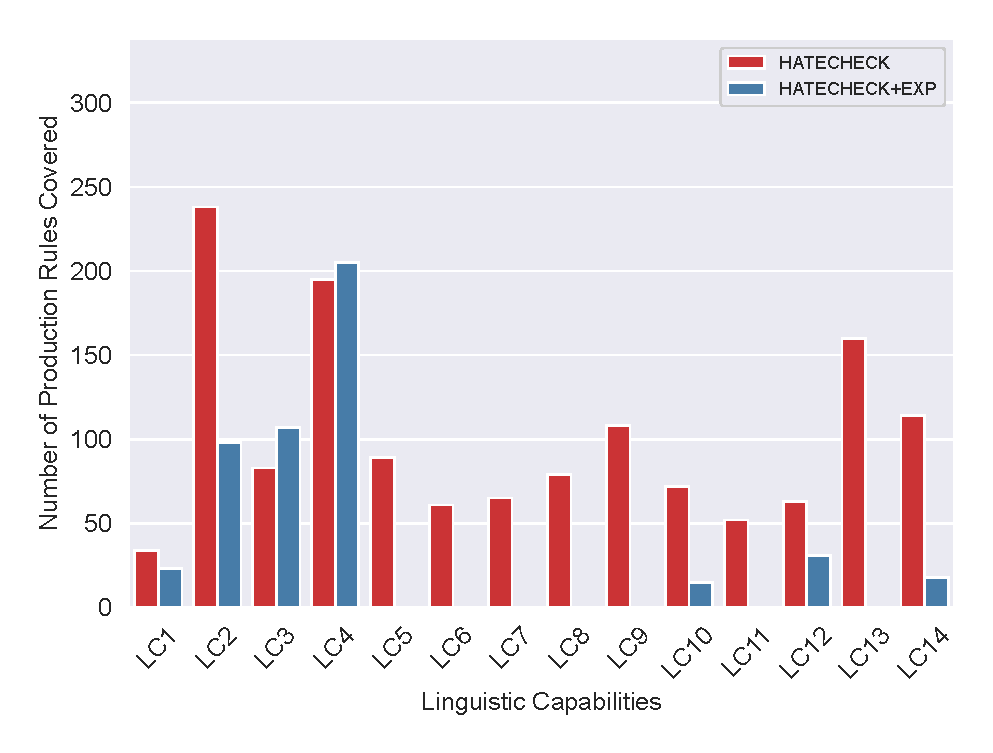
\includegraphics[width=0.45\textwidth]{figs/pdr-hatecheck-barplot.eps}
%     \caption{\PdrBarplotHsFigCaption}
% \end{figure}

% \begin{figure}%
%     \centering
%     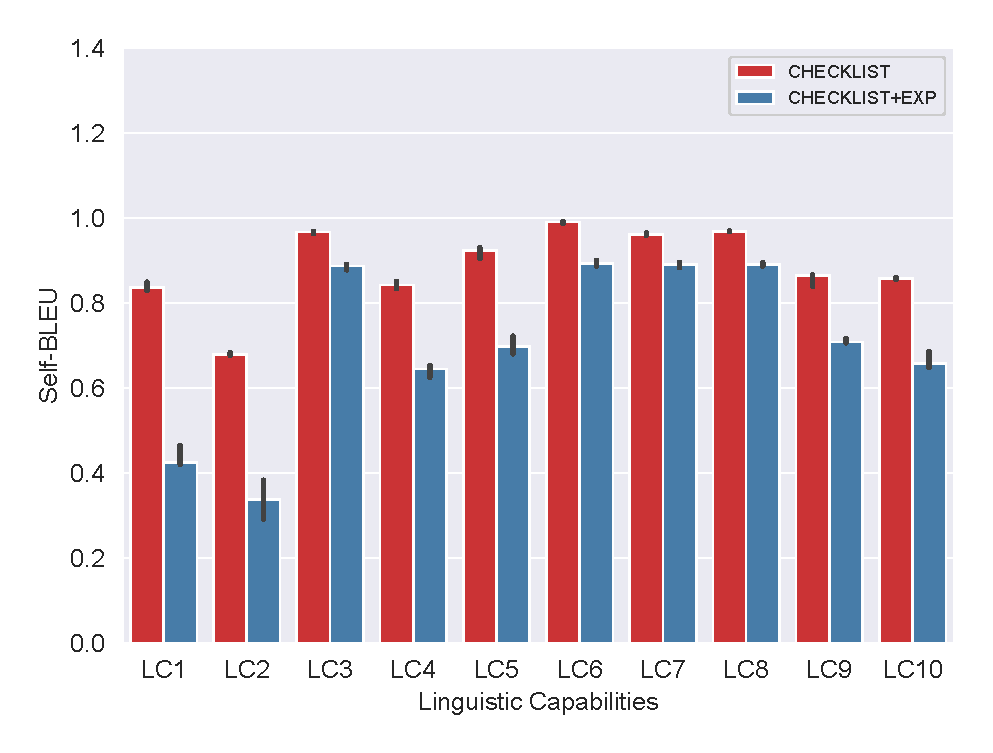
\includegraphics[width=0.4\textwidth]{figs/selfbleu-checklist-barplot.eps}
%     \caption{\SelfbleuBarplotFigCaption}
% \end{figure}

% \begin{figure}%
%     \centering
%     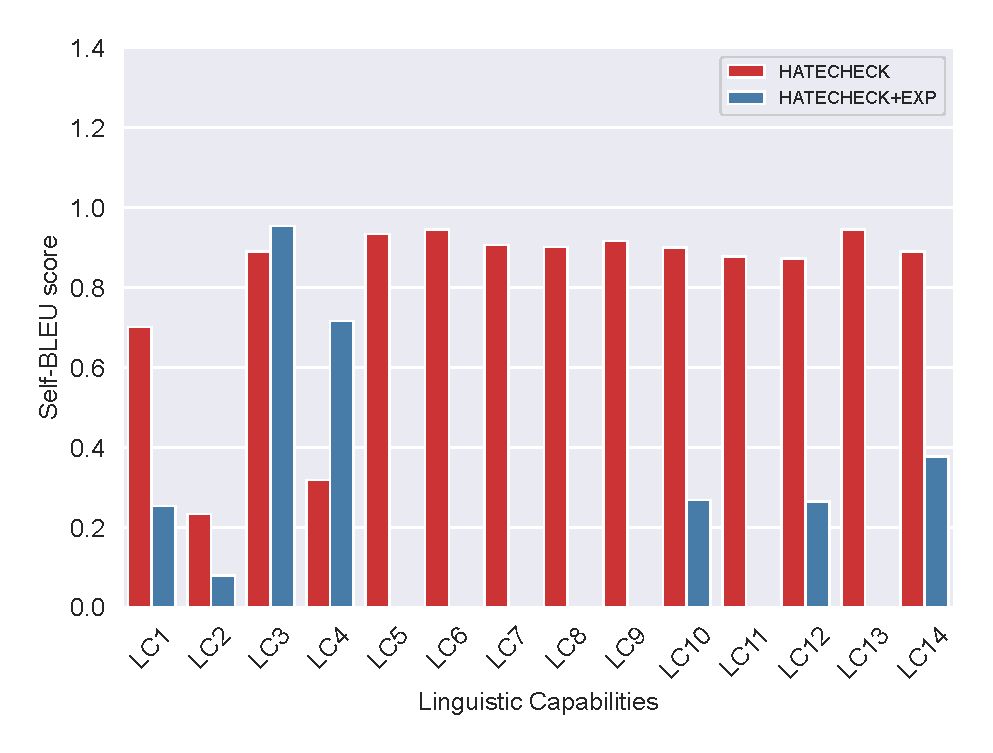
\includegraphics[width=0.45\textwidth]{figs/selfbleu-hatecheck-barplot.eps}
%     \caption{\SelfbleuBarplotHsFigCaption}
% \end{figure}

% \begin{figure}%
%     \centering
%     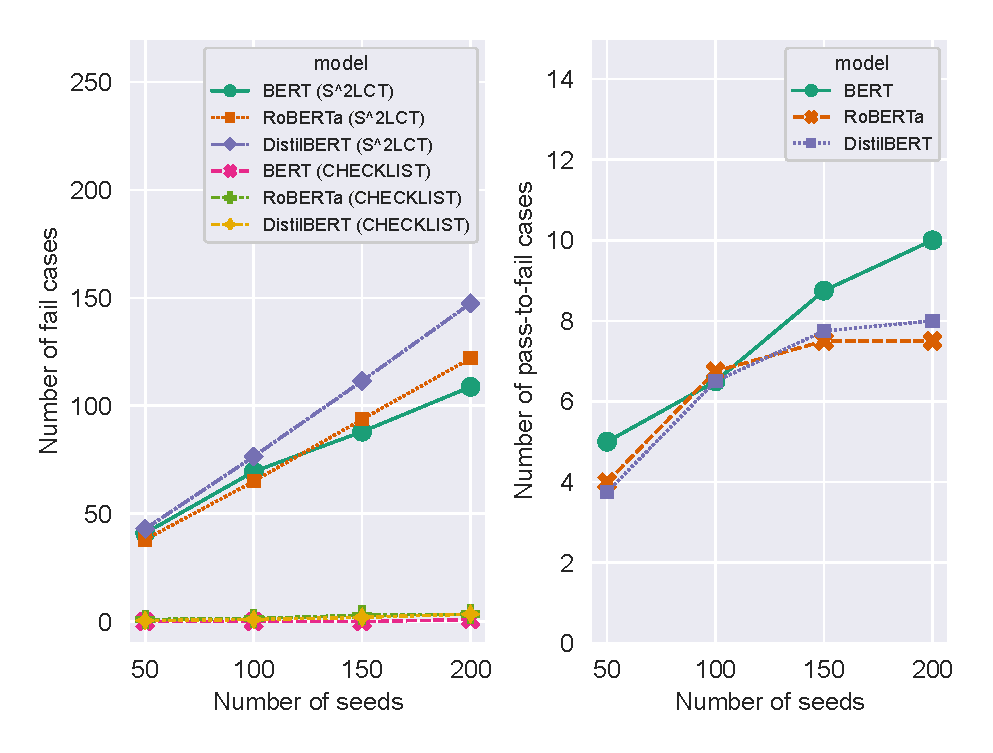
\includegraphics[width=0.35\textwidth]{figs/numfail-pass2fail-agg-lineplot.eps}
%     \caption{\FailModelsFigCaption}
% \end{figure}

% \begin{figure}%
%     \centering
%     \subfloat[][\centering\NumFailModelsSubFigCaption]{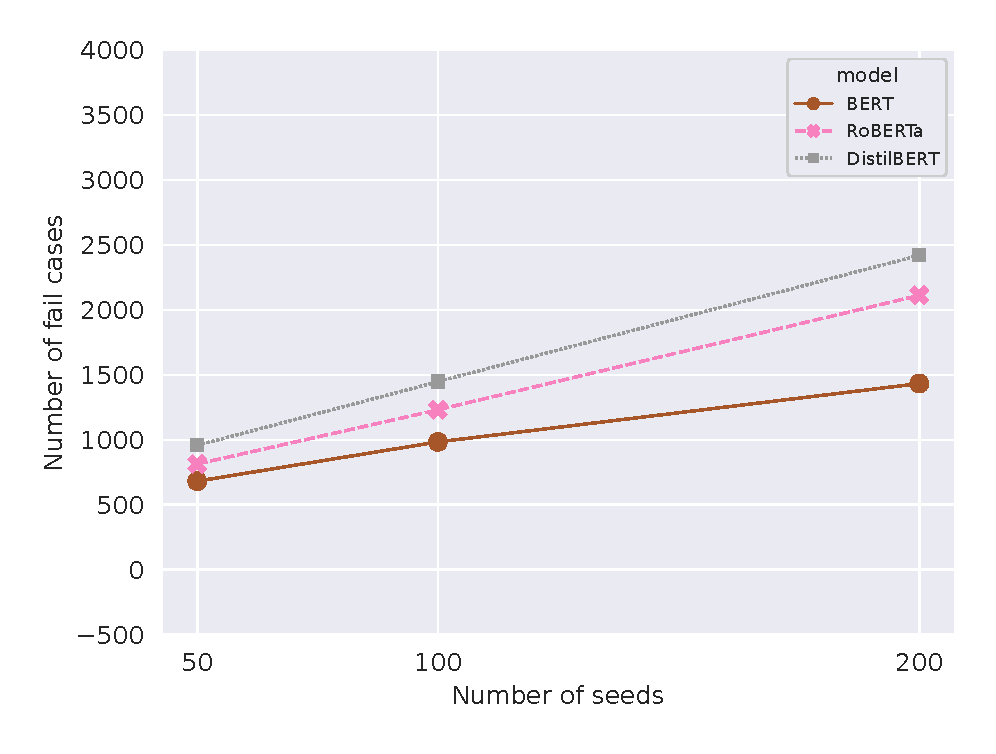
\includegraphics[width=0.35\textwidth]{figs/numfail-agg-lineplot.eps}}%
%     \qquad
%     \subfloat[][\centering\FailRateModelsSubFigCaption]{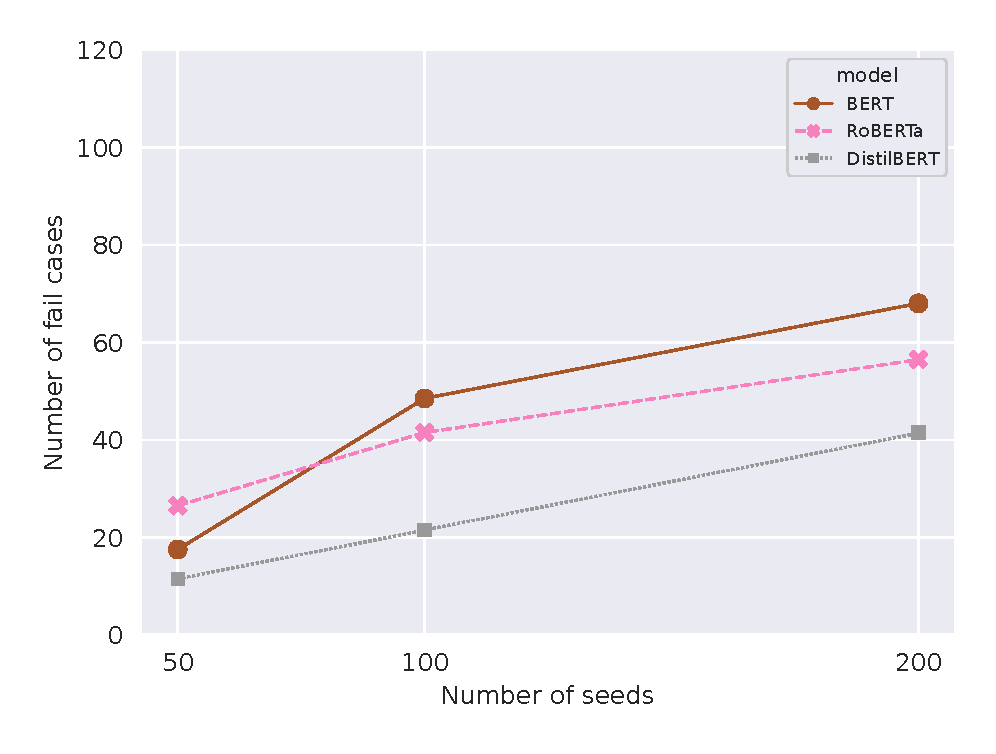
\includegraphics[width=0.35\textwidth]{figs/pass2fail-agg-lineplot.eps}}
%     \caption{\FailModelsFigCaption}
% \end{figure}

\subsection{\ref{rq:one}: Diversity}

% Our results show that \emph{\tool generated many test cases that the sentiment analysis models failed to predict the correct labels, and it produced significantly more diverse test cases than \Cklst did.}
Our results show that \emph{\tool produced test suites with significantly more diversity than \bls did.} 
% In this experiment, we show the test case diversity by comparing \selfbleu and \pdr metrics between \tool and capability-based testing \bls. In addition, we show increase in test case diversity by comparing \selfbleu and \pdr metrics between \tool using \Cklst and \hck as seeds and \Cklst and \hck themselves.

\MyPara{\selfbleu and \Pdr} 
Figure~\ref{fig:PdrSelfbleu} compares the \selfbleu and \pdr scores of the test suite generated by \tool in contrast to those of \Cklst and \hck.
The x-axis shows the sizes of the generated test suite, and the y-axis shows the metric scores.
% Median value of \selcbleu scores are computed from randomly sampled seeds over 3 trials for each \lc,
The figure displays the median \selfbleu and \pdr scores over all \lcs and 5 trials on the left and right, respectively. The results show that \tool's test suite is more diverse than the baselines', with significantly lower \pdr scores and significantly higher \selfbleu scores. This highlights the advantages of searching from a real-world dataset rather than relying on limited preset templates. Furthermore, using expanded sentences in \tool leads to lower \selfbleu and higher \pdr scores, demonstrating the syntax-based expansion of \tool improves sentence diversity.

Figure~\ref{fig:PdrSelfbleuBarplot} shows the \selfbleu and \pdr scores of test suites generated by baseline methods and their expanded versions using \tool. The x-axis shows the method name, and the y-axis shows the corresponding scores across all \lcs. The left sub-figure displays the \selfbleu scores, and the right sub-figure shows the \pdr scores. The results indicate that the expanded \Cklst and \hck achieve better \pdr scores than their original versions, demonstrating the effectiveness of \tool's syntax-based expansion module in increasing the diversity of the generated test suite. Additionally, the expanded \Cklst performs worse in terms of \selfbleu scores, while the expanded \hck has comparable scores to its original version.

Table~\ref{table:MtnlpComp} compares \tool's expanded \sents and \mtnlp for 100 randomly selected seeds. The first column lists the NLP task, and the second column displays the approaches for text generation. Columns 3-5 show the number of generated \sents, \selfbleu, and \pdr scores over 5 sampling trials. \tool generates more \sents than \mtnlp for all tasks and has higher \selfbleu and \pdr scores, demonstrating the effectiveness of \tool's syntax expansion in increasing test case diversity. \mtnlp sometimes fails to mutate seed \sents due to the unavailability of suitable human-related words for mutation.

Table~\ref{table:AdvComp} compares \tool-expanded \sents with adversarial text generation baselines from Section~\ref{sec:experiment_bl}. The first column shows the approach type and the second column shows the number of generated \sents using \tool and the baselines from 50 randomly selected seeds. The third and fourth columns show the \selfbleu and \pdr scores over 5 sampling trials. Results show that Alzantot~\etal~\cite{alzantot2018genadvexp} has the lowest \selfbleu scores, whereas \tool expansion achieves the highest scores in the number of generated \sents and \pdr, introducing various syntax components while maintaining text diversity.



% \paragraph*{\Pdr} Right in figure~\ref{fig:PdrSelfbleu} compares \pdr between the \tool seed sentences, \tool seed and expanded sentences, and the \Cklst test cases. The x-axis shows the sizes of random samples of \tool seed sentences, \tool seed and expanded sentences, and \Cklst test cases, and y-axis shows the \pdr scores. Median of the \pdr scores over all \lcs is shown in the right in the figure~\ref{fig:PdrSelfbleu}. The figure \ref{fig:PdrSelfbleu} shows that \tool seed and/or expanded sentences produce significantly higher \pdr scores than \Cklst test cases did. Also, more \tool seeds cover more production rules because of the increase in diversity obtained from more \tool seeds.

% Figure~\ref{fig:PdrBarplot, HsPdrBarplot} compares the \pdr between all \tool seeds and all \Cklst test cases for each \lc. The x-axis shows each one \lc, and the y-axis is the natural logarithmic scale of \pdr for these test cases.
% % \tool test cases are generated from randomly selected 50 seeds, and the median value over 3 trials for each \lc is reported.
% % It is observed that \tool covers significantly higher number of different syntactic production rules than \Cklst for all \lcs.
% We observed that \tool seeds cover significantly higher number of production rules in each \lc than all \Cklst test cases (ranging from 90 for LC1 to 8518 for LC8 for \tool seeds and from 13 for LC1 to 44 for LC3 for \Cklst seeds) in each \lc.
% % (ranging from 4.92 times to 20.38 times higher scores for LC7 and LC6 respectively) 

% Overall, the above results show that \tool test cases are significantly more diverse with regards to semantic and syntactic structure than \Cklst.


\begin{figure}
    \centering
    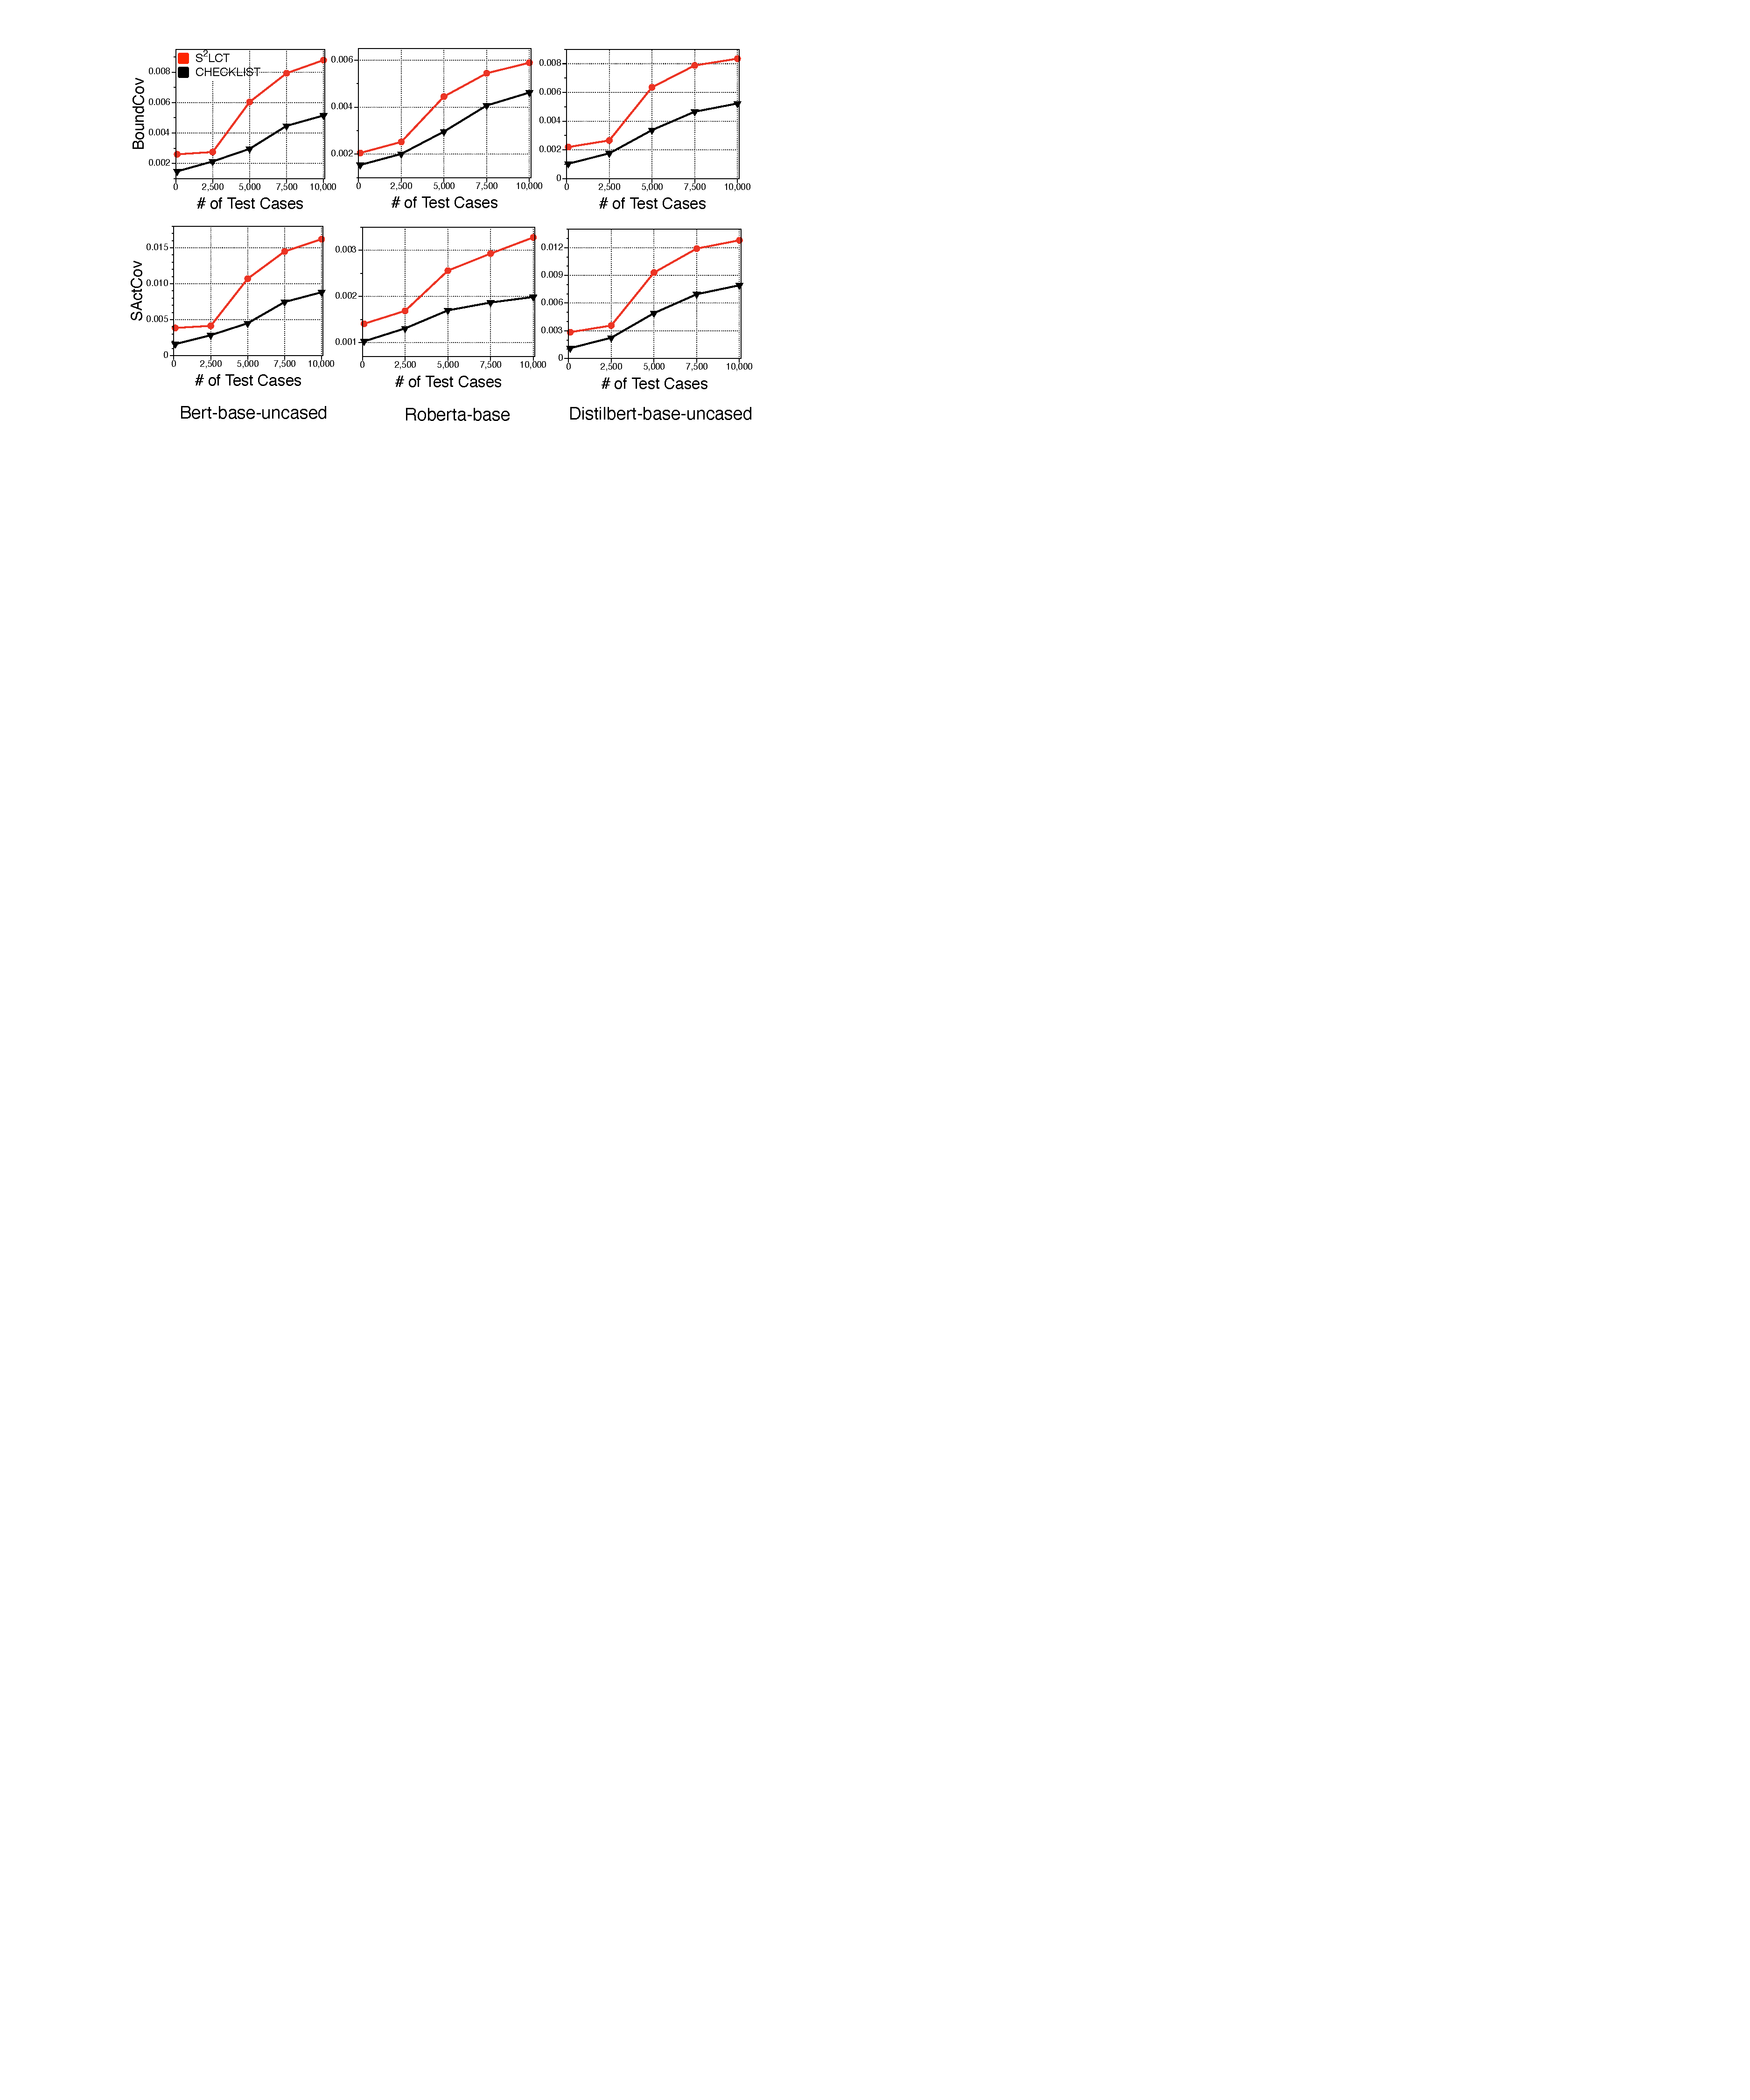
\includegraphics[width=0.5\textwidth]{figs/coverage.pdf}
    \vspace{-4mm}
    \caption{Coverage results of \tool and \Cklst test cases.}
    \label{fig:coverage}
\end{figure}

Next, Figure \ref{fig:coverage} shows the coverage results of \tool and \Cklst test cases. The red line represents \tool coverage and the black line represents \Cklst coverage. Each column in Figure \ref{fig:coverage} represents the results for one NLP model. The first row is the \textit{BoundCov} results and the second row is the \textit{SActCov} results.

We made three observations.
First, for \emph{all} experimental settings (i.e., NLP model and coverage metric), \tool achieves higher coverage than \Cklst. Recall that a higher coverage implies the test cases are more diverse and do not have a similar statistical distribution to the model training data. As a result, a test suite with greater coverage complements the model training data distribution (\ie holdout testing data) better.
For example, for the first NLP model under test, \tool can achieve a higher coverage than \Cklst with only half the number of test cases.
This result confirms that \tool can generate more diverse test cases to complement the holdout dataset for testing NLP models.

Second, as the number of test cases increases, the test suite can achieve better coverage. Such observation is intuitive. However, generating a more extensive test suite is not easy, particularly  for \Cklst, which is a manually template-based approach.

Third, for each NLP model, there is no fixed relationship between \textit{BoundCov} and \textit{SActCov}. In other words, while a test suite may produce higher \textit{BoundCov} for some models, the same test suite may get higher \textit{SActCov} for other NLP models.
Recall that \textit{BoundCov} measures both the upper and lower corner neurons and \textit{SActCov} measures only the upper corner neurons. 
Such observation implies that the upper and lower corner neurons are distributed unevenly, and measuring only one of them is not enough.

\subsection{\ref{rq:two}: Effectiveness}
Our results show that \emph{\tool generates diverse test cases that expose classification errors in NLP models, outperforming the baselines.}
%Specifically, we compared the testing results of \tool with \Cklst for \sa and \hck for \hsd.

\MyPara{The Number of Test Cases}
Table~\ref{table:TestResultAll} and~\ref{table:TestResultHsd} present the results of our effectiveness metrics defined in Section \ref{sec:metric}.  For all \lcs, \tool generates a significant number of test cases, ranging from 70 on LC1 to 533,575 on LC8.
For LC1, LC2, LC4, and LC5, \tool generates fewer test cases than \Cklst because of the small number of seeds. However, the syntax-based sentence expansion phase generated 51 to 503 test cases. In Table~\ref{table:TestResultHsd}, \tool generates more test cases than \hck for every \lcs except LC11, indicating that \tool is more beneficial in generating a sufficient number of test cases. The results show that \tool generates many test cases in the NLP models that fail to predict the correct labels, providing further qualitative test cases than baselines for finding errors.

\MyPara{Fail Rate and Failed Cases}
Figure~\ref{table:TestResultAll} demonstrates that at least one model introduces a higher number of failed test cases on \tool test cases than \Cklst in 7 \lcs, and at least one model achieves a higher failure rate on \tool than on \Cklst in all other \lcs (ranging from 4.27\% to 99.64\%) except for LC8 and LC9. Additionally, in table~\ref{table:TestResultHsd}, we observe that every \lcs for \hsd has a higher number of failed test cases on \tool test cases than \hck, with the failure rate being higher for at least one model in every \lcs except for LC1 and LC5 (ranging from 1.89\% to 88.89\%). Based on these findings, we can conclude that \tool is more effective in generating test cases to identify  errors.

% \paragraph*{Failed Cases}
% Left in figure~\ref{fig:FailModels} compares the numbers of failed cases between \tool and \Cklst. 
% The x-axis shows the sizes of random samples of \tool seed sentences and CHECKLIST test cases, and y-axis shows the number of failed cases. Median number of failed cases from \sa models over \lcs is shown in left in figure~\ref{fig:FailModels}. We observed that \tool seeds introduce more failed cases than \Cklst test cases, and it shows the higher effectiveness of \tool test cases. In addition, it shows that more \tool seeds presents more failed cases, demonstrating the benefit of using more seeds when resource permits.

\MyPara{\Ptf Cases} We observed that many test cases failed in the expanded set but not in their corresponding seeds (as shown in the last column of Table~\ref{table:TestResultAll} and~\ref{table:TestResultHsd}). This type of error case ranges from 0 to 12,729 for \sa and from 0 to 4,365 for \hsd. These results demonstrate that the syntax-based sentence expansion phase effectively introduces more diverse sentence structures, which can potentially expose errors in NLP models that may not be evident in the original seed test cases.

\InputWithSpace{tables/manual-study-table}

\subsection{\ref{rq:three}:  Consistency}


Table~\ref{table:ManualStudy} shows the results of our consistency study. The first column lists the NLP tasks, and the second column distinguishes between seed and expanded sentences. The third column indicates the number of test cases used. Columns 4-6 present the scores of label consistency, LC relevancy, and expansion validity sentences, respectively. Our analysis shows that \emph{\tool generates test cases with high label consistency}, with scores of 0.83 for both seed and expanded test cases for \sa and 0.80 and 0.79 for seed and expanded cases, respectively, for \hsd, indicating that the test oracles constructed by \tool align with human sentiment labeling most of the time.
Moreover, the results show high expansion validity scores of 1.0 for \sa and 0.97 for \hsd, indicating that the tool effectively preserves the semantic meaning of seed sentences during the expansion process. The \lc relevancy score is presented in column 5 of Table \ref{table:ManualStudy}. The result shows that \emph{\tool generates test cases that are correctly categorized to the corresponding \lcs most of the time}. The \lc relevancy scores for the seed and expanded sentences are 0.92 and 0.84 for \sa and \hsd, respectively, achieving high agreement with human assessment. The fact that the expanded sentences generated by \tool have the same level of \lc relevancy as the seed sentences demonstrates that the syntax-based sentence expansion retains the \lcs.












\section{Application of \tool}
\label{sec:application}
% \item \label{rq:four}: \textbf{Usefulness of Test Inputs.} 

In this section, we showcase how \tool can be used in conjunction with explainable ML techniques to assist developers in identifying the root causes of bugs in \sa models.

\begin{figure*}
    \centering
    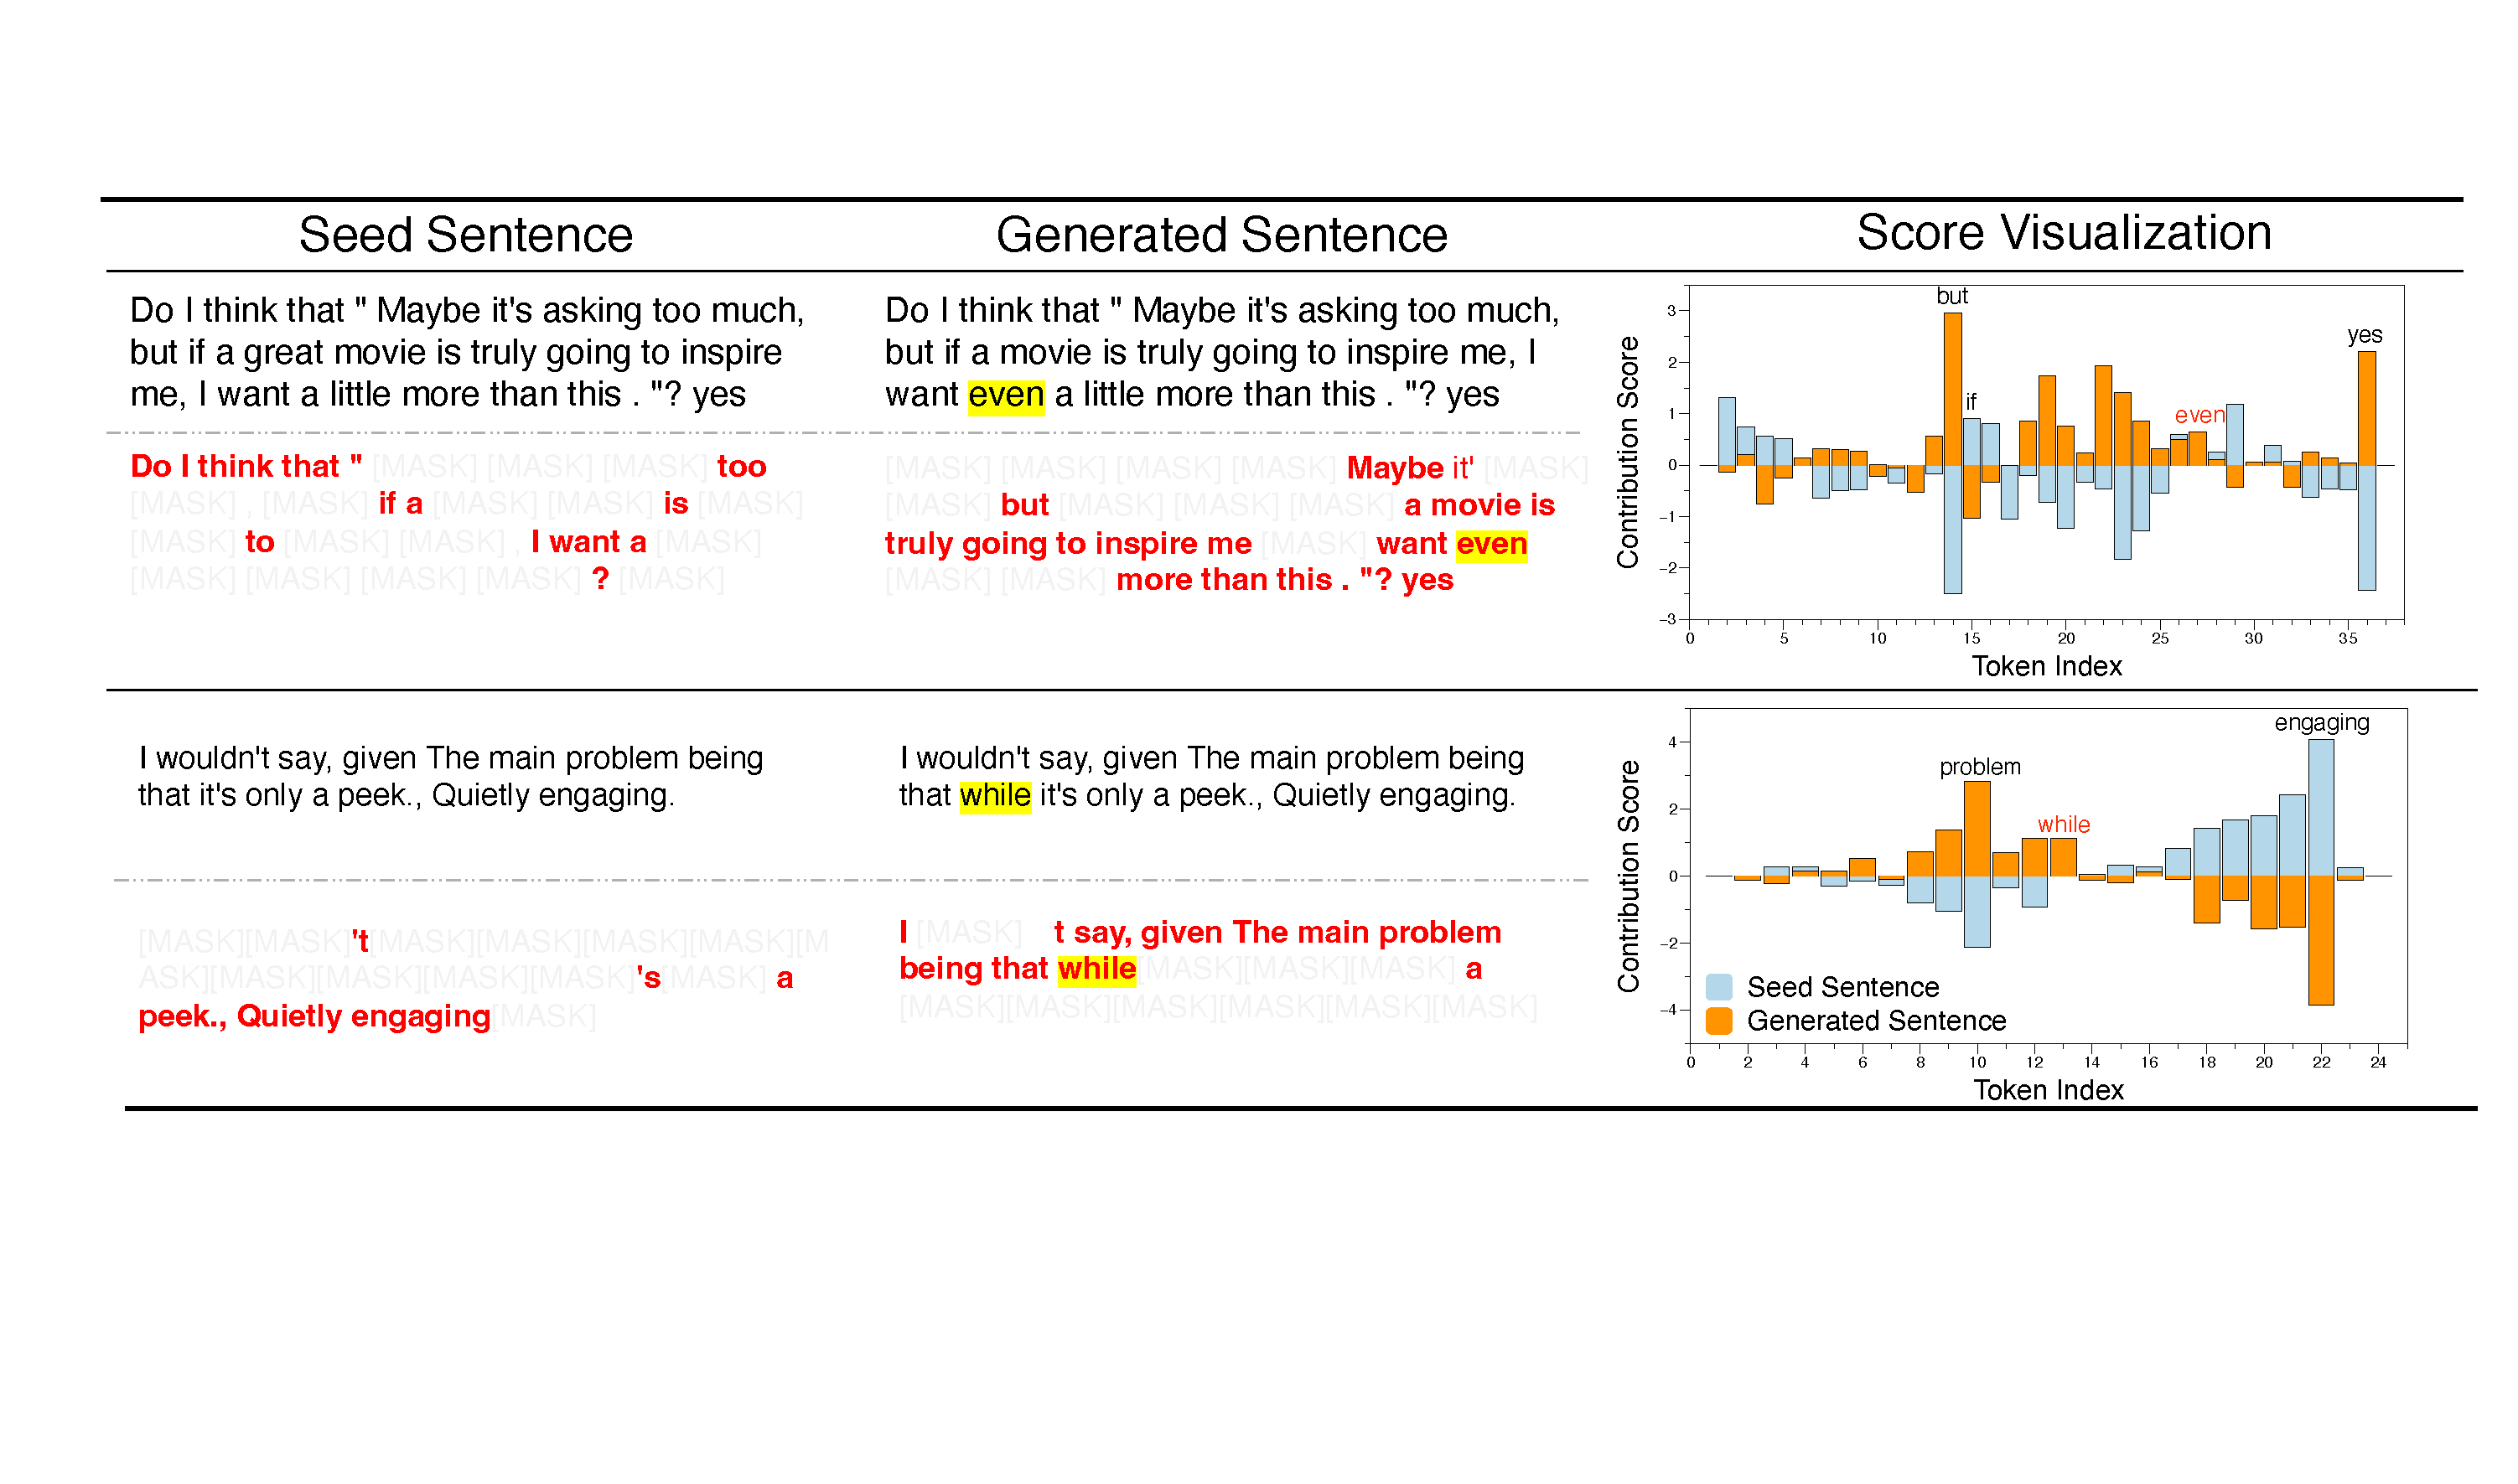
\includegraphics[width=0.7\textwidth]{figs/explain.pdf}
    \vspace{-4mm}
    \caption{Visualization of the buggy reason of two \tool generated test cases.}
    \label{fig:explain}
\end{figure*}


\MyPara{Experimental Process}
we conduct experiments to demonstrate that \tool can help developers understand the bugs in the NLP models.
Recall that \tool generates test cases by mutating seed sentences (\eg by expanding one token in the seed input). Still, it is unclear why mutating one token will cause the model to produce misclassified results.
We seek to help developers understand why such mutation will result in the misclassification. 
Existing work \cite{simin2020denas, lemna, lime} has demonstrated that the ML model prediction is dominated by a minimal set of input features (\ie tokens in input sentences). Motivated by such intuition, we identify a minimal set of input tokens that dominate the model prediction.

Formally, given a input sentence $x = [tk_1, tk_2, \cdots, tk_n]$, and the NLP model under test $f(\cdot)$, our goal is to find a masking template $T = [t_1, t_2, \cdots, t_n]$, where $t_i$ is 0 or 1, representing masking the $i^{th}$ token (\ie $tk_i$) in $x$ or not.
The template $T$ can mask some tokens in $x$ with attribute tokens, and the masked input has a high probability of retaining the original prediction $x$, denoted as
\begin{equation}
    P(f(T(x)) = f(x)) \ge P_{thresh}
    \label{eq:prob}
\end{equation}
To create such a template $T$, we first compute the contribution score of each input token using an existing explainable ML technique \cite{lemna}. We then begin with the full mask template (\ie, all tokens are masked); such full mask template definitely does not satisfy Equation \ref{eq:prob}.
We then iteratively shift one position from mask to non-mask based on the order of each token's contribution score, until the template $T$ satisfies Equation \ref{eq:prob}.
Because we iterate the size of the mask, the generated template $T$ will keep the minimum number of tokens in $x$. Moreover, since the input $x$ is an incorrect prediction, the generated template $T$ is likely to produce misclassification (i.e., the probability to be misclassified is larger than $P_{thresh}$).

\MyPara{Results} We generate a template that dominates the NLP model prediction to assist developers in understanding the false predictions. Figure \ref{fig:explain} shows the generated templates for two randomly selected seeds and their corresponding expanded test inputs.
The first example tests ``sentiments in (question, yes) form'' (LC9), and the second example tests ``negative positive with neutral content in the middle''  (LC7).
The first column shows the seed sentence, the second shows the expanded sentence, and the third shows each token's contribution score. The blue bar indicates the score for seed inputs, whereas the orange bar reflects the score for the expanded sentences.
We highlight the mutated token with yellow background and generated templates with red text. 

The results show that after mutating the seed sentence with one token, the token set that dominates the NLP model prediction has changed.
We can trace the root causes to the bias of the training data on the \lc under test; as a result, for the \lc under test, the model has a bias towards positive/negative for certain token sequence patterns. For example, LC9 has a bias toward the token sequence pattern that includes "maybe .... but ... even... yes". Thus, adding the token ``even" to the seed sentence will match one of those biased sequence patterns.
Sentences with such pattern in the training dataset are dominantly positive; thus, the models make the wrong decision on the sentence with ``even'' as positive. 
The visualization of each token's contribution score in the third column confirms our observation. Once ``even'' is added, scores of other tokens such as ``but'' and ``yes'' all change from negative to positive.
To fix the issue for LC9, we need to add more negative training samples with the format of ``maybe . .. but ... even ... yes''.
%he experimental results in Fig. \ref{fig:explain} illustrate that \tool can help developers to understand the buggy reason of the misclassification go no在,